\documentclass{report} 

\usepackage{graphicx}

\begin{document}  

%============================%
%                            %
%   Cholesky factorization   %
%                            %
%============================%
\section{Cholesky factorization}

%----------------%
%    Cholesky    %
%----------------%
\begin{figure}[ht]
  \centering
  \setlength{\unitlength}{1mm}
  \begin{picture}(60,60)(0,0)
%-> \thicklines\put(0,0){\framebox(63,80){}}
    \put( 1,0){\includegraphics[height=6.0cm]{Cholesky.eps}}
  \end{picture}
\end{figure}

\begin{equation}
  \begin{array}{ll}
    \mbox{\bf Row 1}       & \mbox{\bf Row 2}                       \\
    A_{11} = L_{11}^2      & A_{22} = L_{12}^2      + L_{22}^2      \\
    A_{12} = L_{12} L_{11} & A_{23} = L_{12} L_{13} + L_{22} L_{23} \\
    A_{13} = L_{13} L_{11} & A_{24} = L_{12} L_{14} + L_{22} L_{24} \\
    A_{14} = L_{14} L_{11} &                                        \\ 
                           &                                        \\
    \mbox{\bf Row 3}                                       & \; \mbox{\bf Row 4}                                   \\
    A_{33} = L_{13}^2 + L_{23}^2 + L_{33}^2                & \; A_{44} = L_{14}^2 + L_{24}^2 + L_{34}^2 + L_{44}^2 \\
    A_{34} = L_{13} L_{14} + L_{23} L_{24} + L_{33} L_{34} & \; 
  \end{array}
\end{equation}

\begin{equation}
  \begin{array}{ll}
    \mbox{\bf Row 1}         & \mbox{\bf Row 2}                         \\
    L_{11} = \sqrt{A_{11}}   & L_{22} = \sqrt{A_{22} - L_{12}^2}        \\
    L_{12} = A_{12} / L_{11} & L_{23} = (A_{23} - L_{12} L_{13})/L_{22} \\
    L_{13} = A_{13} / L_{11} & L_{24} = (A_{24} - L_{12} L_{14})/L_{22} \\
    L_{14} = A_{14} / L_{11} &                                          \\ 
                             &                                          \\
    \mbox{\bf Row 3}                                         & \; \mbox{\bf Row 4}                                        \\
    L_{33} = \sqrt{A_{33} - L_{13}^2 - L_{23}^2}             & \; L_{44} = \sqrt{A_{44} - L_{14}^2 - L_{24}^2 - L_{34}^2} \\
    L_{34} = (A_{34} - L_{13} L_{14} - L_{23} L_{24})/L_{33} & \; 
  \end{array}
\end{equation}

\clearpage

%=======================================%
%                                       %
%   Incomplete Cholesky factorization   %
%                                       %
%=======================================%
\section{Incomplete Cholesky factorization}

%-----------------------%
%  Incomplete Cholesky  %
%-----------------------%
\begin{figure}[ht]
  \centering
  \setlength{\unitlength}{1mm}
  \begin{picture}(60,60)(0,0)
%-> \thicklines\put(0,0){\framebox(63,80){}}
    \put( 1,0){\includegraphics[height=6.0cm]{Incomplete_Cholesky.eps}}
  \end{picture}
\end{figure}

\begin{equation}
  \begin{array}{ll}
    \mbox{\bf Row 1}       & \mbox{\bf Row 2}                       \\
    A_{11} = L_{11}^2      & A_{22} = L_{12}^2      + L_{22}^2      \\
    A_{12} = L_{12} L_{11} & A_{23} = L_{22} L_{23}                 \\
    A_{13} = 0             & A_{24} = 0                             \\
    A_{14} = 0             &                                        \\ 
                           &                                        \\
    \mbox{\bf Row 3}             & \; \mbox{\bf Row 4}              \\
    A_{33} = L_{23}^2 + L_{33}^2 & \; A_{44} = L_{34}^2 + L_{44}^2  \\
    A_{34} = L_{33} L_{34}       & \; 
  \end{array}
\end{equation}

\begin{equation}
  \begin{array}{ll}
    \mbox{\bf Row 1}         & \mbox{\bf Row 2}                  \\
    L_{11} = \sqrt{A_{11}}   & L_{22} = \sqrt{A_{22} - L_{12}^2} \\
    L_{12} = A_{12} / L_{11} & L_{23} = A_{23}/L_{22}            \\
    L_{13} = 0               & L_{24} = 0                        \\
    L_{14} = 0               &                                   \\ 
                             &                                   \\
    \mbox{\bf Row 3}                  & \; \mbox{\bf Row 4}                  \\
    L_{33} = \sqrt{A_{33} - L_{23}^2} & \; L_{44} = \sqrt{A_{44} - L_{34}^2} \\
    L_{34} = A_{34}/L_{33}            & \; 
  \end{array}
\end{equation}

\clearpage

%================================================%
%                                                %
%   General cartesian system, compass notation   %
%                                                %
%================================================%
\section{General cartesian system, compass notation}

Two-dimensional grid on this figure:

%------------------%
%  Cartesian grid  % 
%------------------%
\begin{figure}[ht]
  \centering
  \setlength{\unitlength}{1mm}
  \begin{picture}(80,40)(0,0)
%-> \thicklines\put(0,0){\framebox(63,80){}}
    \put( 1,0){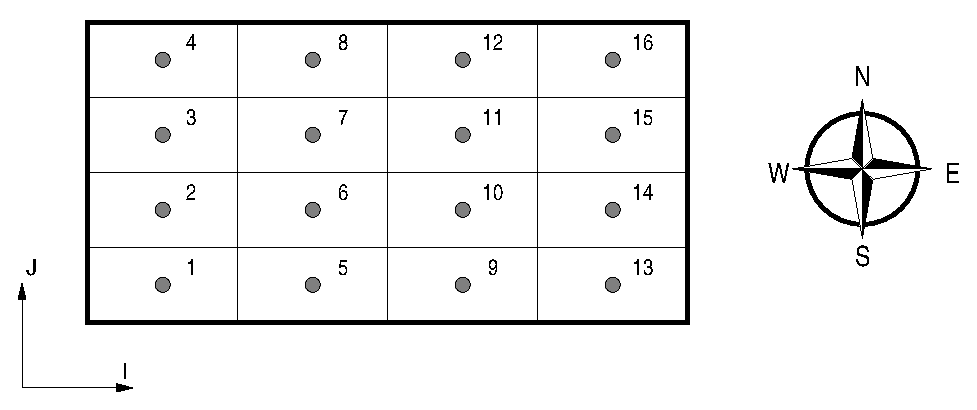
\includegraphics[height=4.0cm]{Grid.eps}}
  \end{picture}
\end{figure}

gives the matrix system with the following topology:

%-------------------------------%
%  Incomplete Cholesky Compass  % 
%-------------------------------%
\begin{figure}[ht]
  \centering
  \setlength{\unitlength}{1mm}
  \begin{picture}(80,80)(0,0)
%-> \thicklines\put(0,0){\framebox(63,80){}}
    \put( 1,0){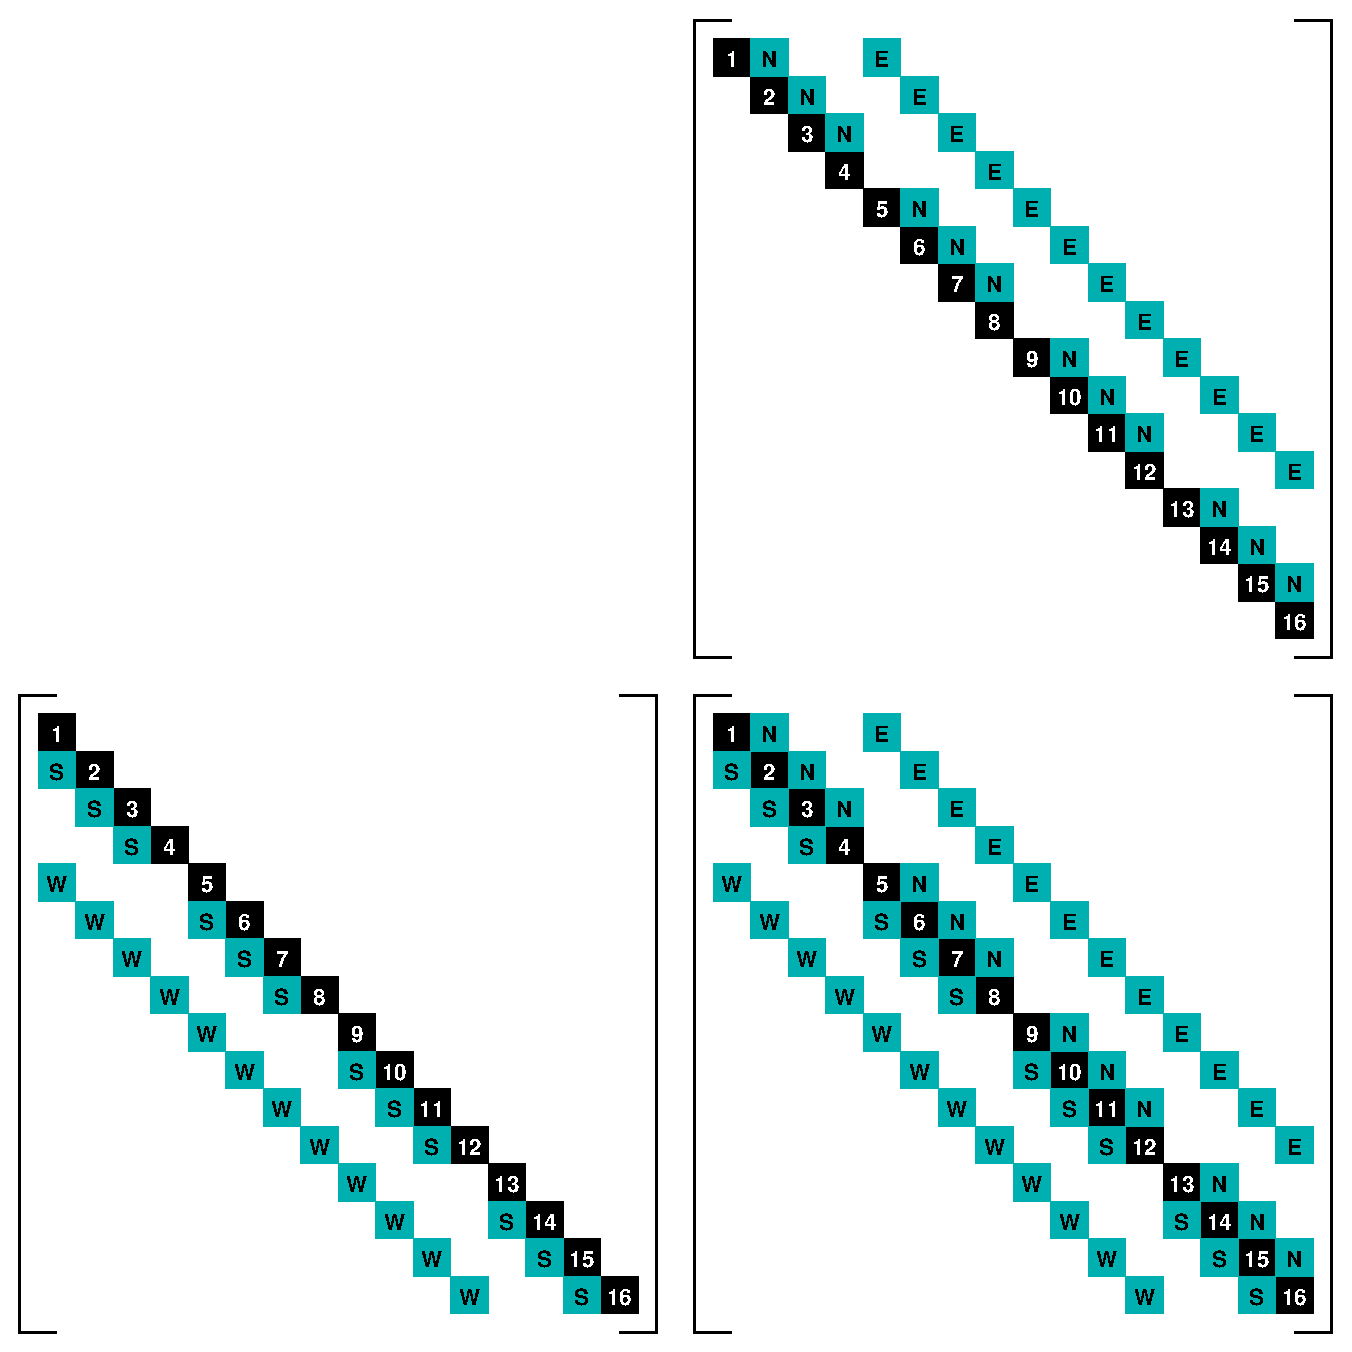
\includegraphics[height=8.0cm]{Incomplete_Cholesky_Compass_2.eps}}
  \end{picture}
\end{figure}

Diagonal entries of the L matrix ($B, S, W < i$):

\begin{eqnarray}
  L_{C,i} = \sqrt{A_{C,i} - L_{B,i}^2 - L_{S,i}^2 - L_{W,i}^2} \\
  L_{B,i} = A_{B,i} / L_{C,i}                                  \\
  L_{S,i} = A_{S,i} / L_{C,i}                                  \\
  L_{W,i} = A_{W,i} / L_{C,i}
\end{eqnarray}

Obviuousy, it is enough to store diagonal entries of the L matrix.

%==================================================%
%                                                  %
%   Solution of linear system with factorization   %
%                                                  %
%==================================================%
\section{Solution of linear system with factorization}

%======================%
%   LU decomposition   %
%======================%
\subsection{LU decomposition}

\begin{equation}
  \bf{A} \bf{x} = \bf{b}
\end{equation}

\begin{equation}
  \bf{A} = \bf{L} \bf{U}
\end{equation}

\begin{equation}
  \bf{L} \underbrace{\bf{U} \bf{x}}_y  = \bf{b}
\end{equation}

Forward solve:

\begin{equation}
  \bf{L} y  = \bf{b}
\end{equation}

Backward solve:

\begin{equation}
  \bf{U} x  = \bf{y}
\end{equation}

%============================%
%   Cholesky decomposition   %
%============================%
\subsection{Cholesky decomposition}

\begin{equation}
  \bf{A} \bf{x} = \bf{b}
\end{equation}

\begin{equation}
  \bf{A} = \bf{L} \bf{L}^T
\end{equation}

\begin{equation}
  \bf{L} \underbrace{\bf{L}^T \bf{x}}_y  = \bf{b}
\end{equation}

\subsubsection{Forward solve}

%-----------%
%  Forward  %
%-----------%
\begin{figure}[h!]
  \centering
  \setlength{\unitlength}{1mm}
  \begin{picture}(60,30)(0,0)
%-> \thicklines\put(0,0){\framebox(63,80){}}
    \put( 1,0){\includegraphics[height=3.0cm]{Forward.eps}}
  \end{picture}
\end{figure}

\begin{equation}
  \bf{L} y  = \bf{b}
\end{equation}

\begin{eqnarray}
  i & = & 1 \rightarrow N \\
  y_i  & = & (b_i - L_{B,i}y_{B,i} - L_{S,i}y_{S,i} - L_{W,i}y_{W,i}) / L_{c,i}
\end{eqnarray}

\subsubsection{Backward solve}

%------------%
%  Backward  %
%------------%
\begin{figure}[h!]
  \centering
  \setlength{\unitlength}{1mm}
  \begin{picture}(60,30)(0,0)
%-> \thicklines\put(0,0){\framebox(63,80){}}
    \put( 1,0){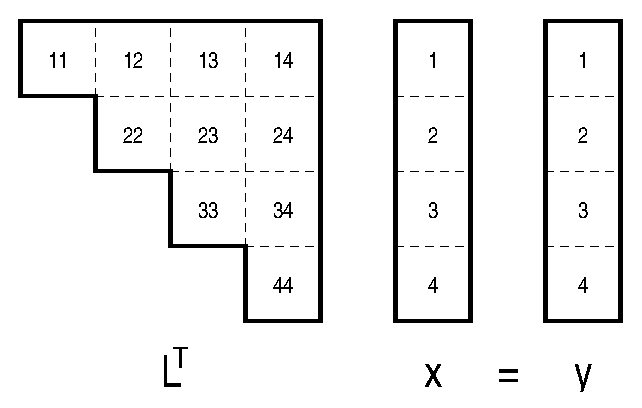
\includegraphics[height=3.0cm]{Backward.eps}}
  \end{picture}
\end{figure}

\begin{equation}
  \bf{L}^T x  = \bf{y}
\end{equation}

\begin{eqnarray}
  i & = & N \rightarrow 1 \\
  x_i  & = & (y_i - L_{T,i}x_{T,i} - L_{N,i}x_{N,i} - L_{E,i}x_{E,i}) / L_{c,i}
\end{eqnarray}

%=========================================================================%
%                                                                         %
%   General cartesian system, compass notation, periodic in i direction   %
%                                                                         %
%=========================================================================%
\section{General cartesian system, compass notation, periodic}

%-------------------------------%
%  Incomplete Cholesky Compass  % 
%-------------------------------%
\begin{figure}[ht]
  \centering
  \setlength{\unitlength}{1mm}
  \begin{picture}(80,80)(0,0)
%-> \thicklines\put(0,0){\framebox(63,80){}}
    \put( 1,0){\includegraphics[height=8.0cm]{Incomplete_Cholesky_Compass_3.eps}}
  \end{picture}
\end{figure}

\end{document}
